\newpage
\subsection{Outliers in Hessian Eigenspectrum}
\label{sec:appendix_M_struct}
One characteristic of Hessian that has been mentioned by many is the outliers in the spectrum of eigenvalues. \citet{sagun2017empirical} suggests that there is a gap in Hessian eigenvalue distribution around the number of classes $c$ in most cases, where $c=10$ in our case. A popular theory to explain the gap is the class / logit clustering of the logit gradients \citep{fort2019emergent, papyan2019measurements, papyan2020traces}. 
Note that these explanations can be consistent with our heuristic formula for the top eigenspace of output Hessian at initialization\--- in the two-layer setting we considered the logit gradients are indeed clustered.

In the layer-wise setting, the clustering claim can be formalized as follows: For each class $k\in[c]$ and logit entry $l\in[c]$, with $\mQ$ be defined as in  \equationref{eqn:app_qx}, and $(\rvx, \ry)$ as the input, label pair, let
\begin{equation}
    \mDelta_{i,j} = \E\left[\left.\mQ_{\rvx}\frac{\partial \vz_{\rvx}}{\partial \vw^{(p)}_j}\right\vert\ervy=i\right].
\end{equation}
Then at the initialization, for each logit entry $j$, $\{\mDelta_{i,j}\}_{i\in[c]}$ is clustered around the ``logit center'' $\hat{\mDelta}_j \triangleq \E_{i\in[c]}[\mDelta_{i,j}]$; at the minima, for each class $i$, $\{\mDelta_{i,j}\}_{j\in[c]}$ is clustered around the ``class center''  $\hat{\mDelta}_i \triangleq \E_{j\in[c]}[\mDelta_{i,j}]$. With the decoupling conjectures, we may also consider similar claims for output Hessians, where
\begin{equation}
    \mGamma_{i,j} = \E\left[\left.\mQ_{\rvx}\frac{\partial \vz_{\rvx}}{\partial {\vz^{(p)}_{\rvx}}_j}\right\vert\ervy=i\right].
\end{equation}
A natural extension of the clustering phenomenon on output Hessians is then as follows: At the initialization, for each logit entry $j$, $ \{\mGamma_{i,j}\}_{i\in[c]}$ is clustered around $\hat{\mGamma}_j \triangleq\E_{i\in[c]}[\mGamma_{i,j}]$; at the minima, for each class $i$, $\{\mGamma_{i,j}\}_{j\in[c]}$ is clustered around $\hat{\mGamma}_i \triangleq \E_{j\in[c]}[\mGamma_{i,j}]$.
Note that we have the layer-wise Hessian and layer-wise output Hessian satisfying
\begin{equation}
    \mH_\Ls(\vw^{(p)}) = \mathop{\E}_{i,j\in[c]}[\mDelta_{i,j}^\T\mDelta_{i,j}],\ \  \mM^{(p)} = \mathop{\E}_{i,j\in[c]}[\mGamma_{i,j}^\T\mGamma_{i,j}].
\end{equation}
 %\textcolor{red}{Rong: Please check if this sentence makes sense}

\paragraph{Low-rank Hessian at Random Initialization and Logit Gradient Clustering}\text{} \\
We first briefly recapture our explanation on the low-rankness of Hessian at random initialization. In \sectionref{sec:theoretical} and \sectionref{sec:detailed-proof}, we have shown that for a two layer ReLU network with Gaussian random initialization and Gaussian random input, the output hessian of the first layer $\mM^{(1)}$ is approximately $\frac{1}{4}\mW^{(2)T}\mA\mW^{(2)}$. We then heuristically extend this approximation to a randomly initialized $L$-layer network, that with $\mS^{(p)} = \mW^{(L)}\mW^{(L-1)}\cdots\mW^{(p+1)}$, the output Hessian of the $p$-th layer $\mH^{(p)}$ can be approximated by $\Tilde{\mM}^{(p)}$ where
\begin{equation}
    \label{eqn:M_SAS_Approx}
    \Tilde{\mM}^{(p)} \triangleq \frac{1}{4^{L-p}}\mS^{(p)T}\mA\mS^{(P)}.
\end{equation}
Since $\mA$ is strictly rank $c-1$ with null space of the all-one vector, $\mH^{(p)}$ is strictly rank $c-1$. Thus $\mH^{(p)}$ is approximately rank $c-1$, and so is the corresponding layerwise Hessian according to the decoupling conjecture.

Now we discuss the connection between our analysis with the theory of logit gradient clustering. As previously observed by \citet{papyan2019measurements}, for each logit entry $l$, $\{\mDelta_{i,j}\}_{l\in[c]}$ are clustered around the logit gradients $\E_{l\in[c]}[\mDelta_{i,j}]$. Similar clustering effects for $\{\mGamma_{i,j}\}_{l\in[c]}$ were also empirically observed by our experiments. Moreover, through the approximation above and the decoupling conjecture, for each logit entry $j$, the cluster centers $\hat{\mGamma}_j$ and $\hat{\mDelta}_j$ can be approximated by
\begin{equation}
\begin{split}
    \hat{\mGamma}_j \approx \Breve{\mGamma}_j &\triangleq (\mS^\T\mQ)_j\\ \hat{\mDelta}_j \approx \Breve{\mDelta}_j &\triangleq ((\E[\vx]\otimes\mS^\T)\E[\mQ])_j.
\end{split}
\end{equation}

Following \citet{papyan2019measurements}, we used t-SNE \citep{vanDerMaaten2008} to visualize the logit gradients. As we see in \figureref{fig:tsne1}, the ``logit centers'' of the clustering directly corresponds to the approximated dominating eigenvectors of the Hessian, which is consistent with our analysis.

\paragraph{Gradient Clustering at Minima}

Currently our theory does not provide an explanation to the low rank structure of Hessian at the minima. However we have observed that the class clustering of logit gradients does not universally apply to all models at the minima, even when the models have around $c$ significant large eigenvalues. As shown in \figureref{fig:tsne2}, the class clustering is very weak but there are still around $c$ significant large eigenvalues. We conjecture that the class clustering of logit gradients may be a sufficient but not necessary condition for the Hessian to be low rank at minima.

% \begin{figure}[H]
%     \centering
%     \subfigure[\centering\small{Eigenspectrum of $\E[\mM]$ at initialization.}]{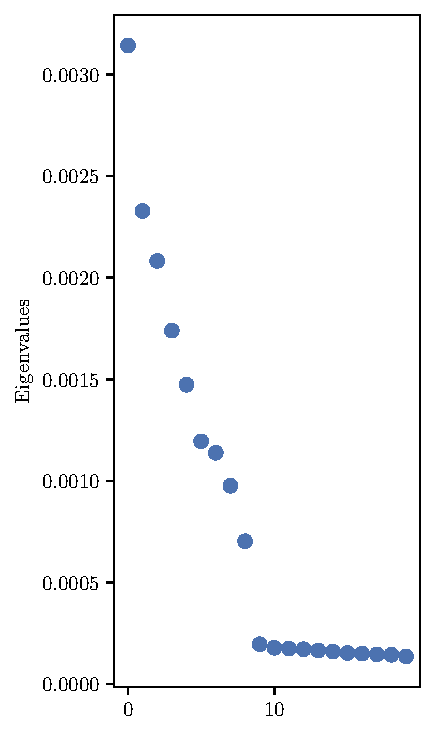
\includegraphics[width=0.25\linewidth]{Appendix_Figures/TSNE_M/new/spec_0.pdf}}
%     \subfigure[\centering\small{Clustering of $\mDelta$ with logits at initialization.}]{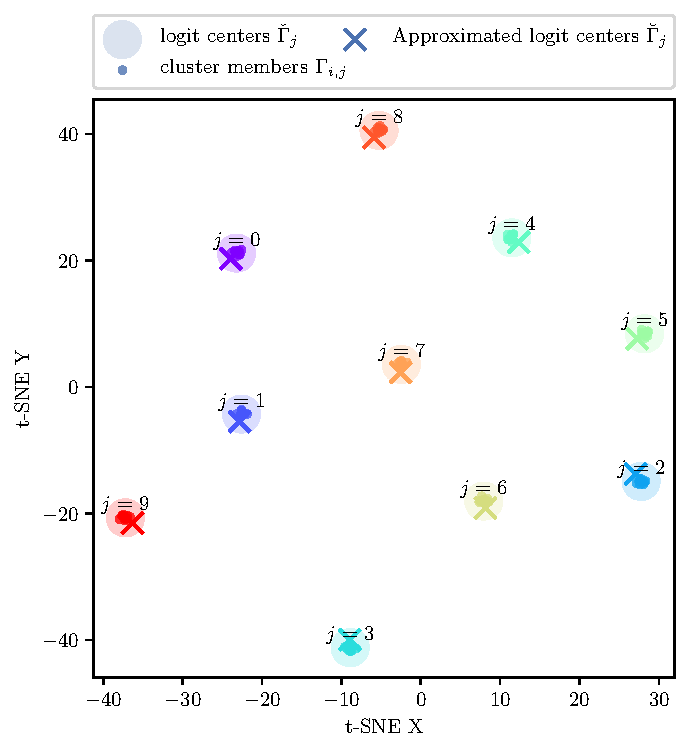
\includegraphics[width=0.36\linewidth]{Appendix_Figures/TSNE_M/new/E0_gamma_ccp_cluster_pred_fc1.pdf}}
%     \subfigure[\centering\small{Clustering of $\mGamma$ with logits at initialization.}]{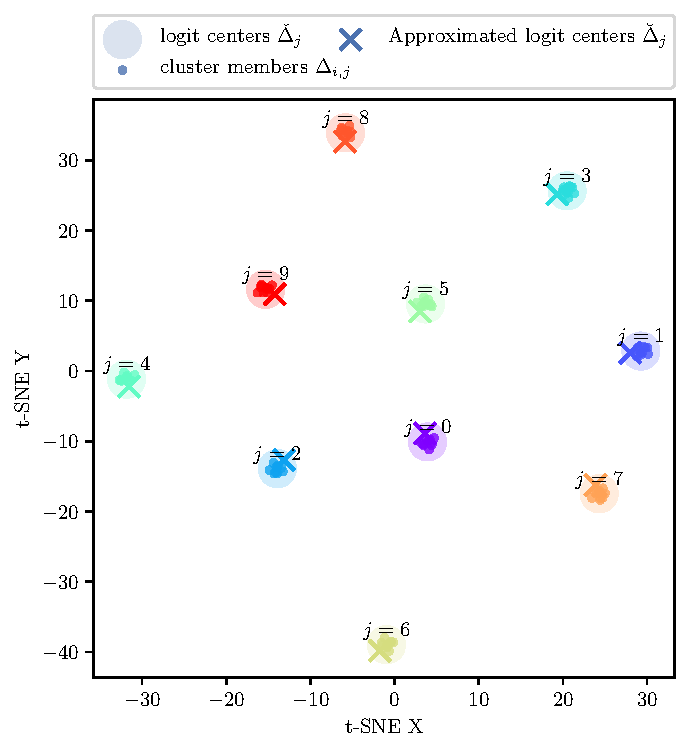
\includegraphics[width=0.36\linewidth]{Appendix_Figures/TSNE_M/new/E0_delta_ccp_cluster_pred_fc1.pdf}}
%     \caption{Logit clustering behavior of $\mDelta$ and $\mGamma$ at initialization (fc1:T-$200^2$)}
%     \label{fig:tsne1}
% \end{figure}
\begin{figure}[h]
    \centering
    \begin{subfigure}[b]{0.2\textwidth}
        \centering
        \captionsetup{justification=centering}
        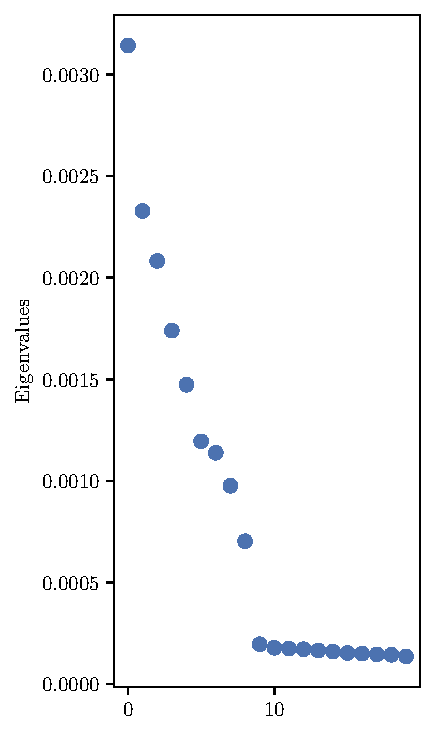
\includegraphics[width=\textwidth]{Appendix_Figures/TSNE_M/new/spec_0.pdf}
        \caption{Eigenspectrum of $\E[\mM]$ at initialization.}
        \label{fig:app_tsne_h_init}
    \end{subfigure}%
    \begin{subfigure}[b]{0.4\textwidth}
        \centering
        \captionsetup{justification=centering}
        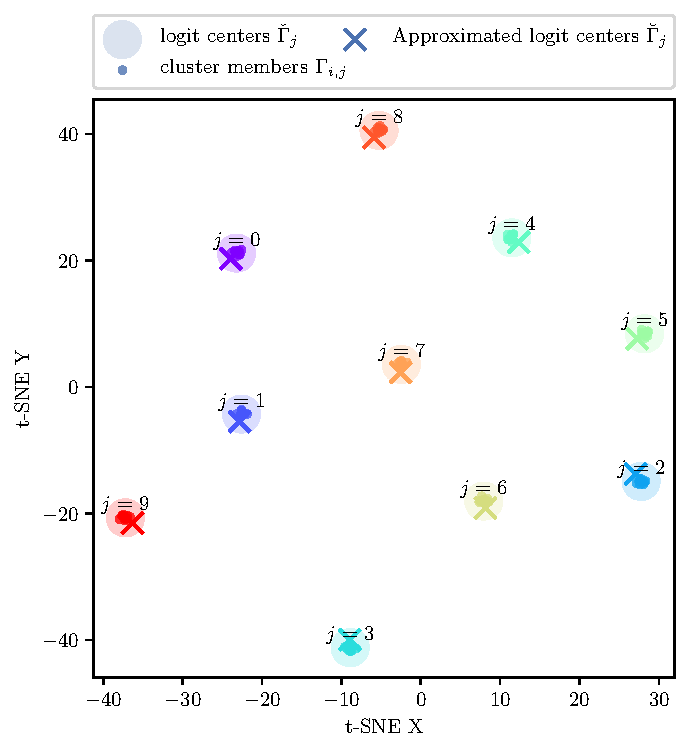
\includegraphics[width=\textwidth]{Appendix_Figures/TSNE_M/new/E0_gamma_ccp_cluster_pred_fc1.pdf}
        \caption{Clustering of $\mGamma$ with logits at initialization.}
        \label{fig:app_tsne_h_min}
    \end{subfigure}%
    \begin{subfigure}[b]{0.4\textwidth}
        \centering
        \captionsetup{justification=centering}
        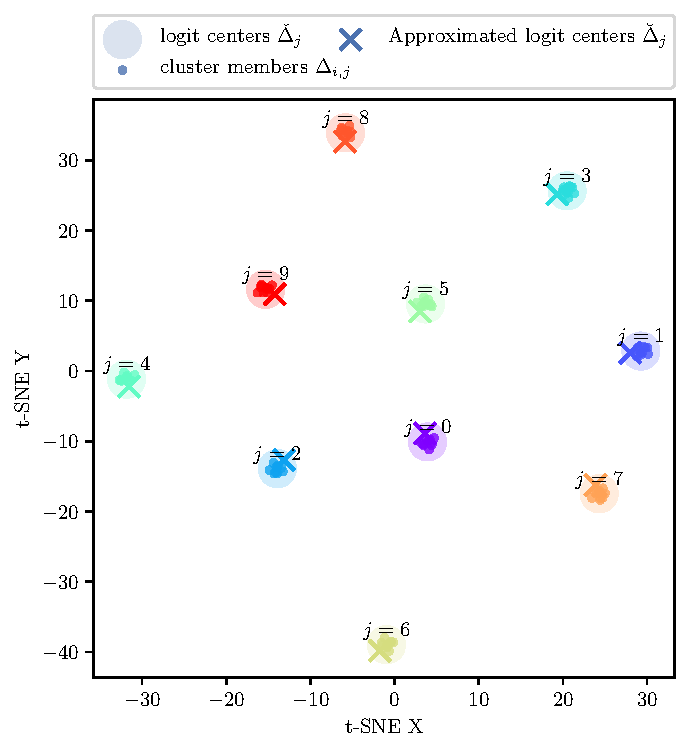
\includegraphics[width=\textwidth]{Appendix_Figures/TSNE_M/new/E0_delta_ccp_cluster_pred_fc1.pdf}
        \caption{Clustering of $\mDelta$ with logits at initialization.}
        \label{fig:app_tsne_m_init}
    \end{subfigure}%
    \captionsetup{justification=centering}
    \caption{Logit clustering behavior of $\mDelta$ and $\mGamma$ at initialization (fc1:T-$200^2$)}
    \label{fig:tsne1}
\end{figure}

% \begin{figure}[H]
%     \centering
%     \subfigure[\centering\small{Eigenspectrum of $\E[\mM]$ at initialization.}]{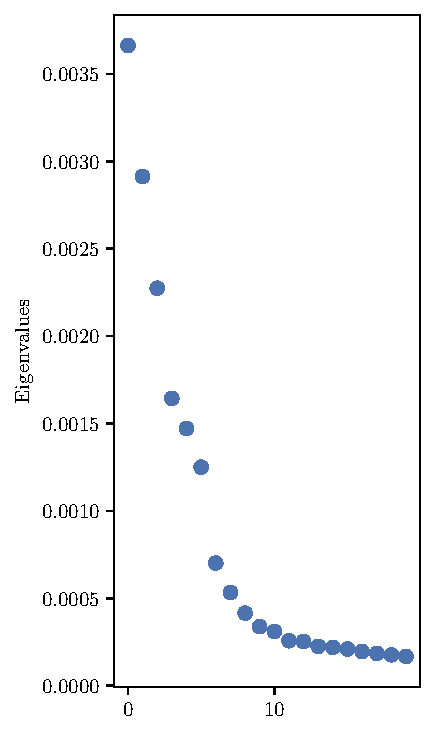
\includegraphics[width=0.25\linewidth]{Appendix_Figures/TSNE_M/new/spec_E-1_gamma_ccp_cluster_pred_fc1.pdf}}
%     \subfigure[\centering\small{Clustering of $\mGamma$ with logits at initialization.}]{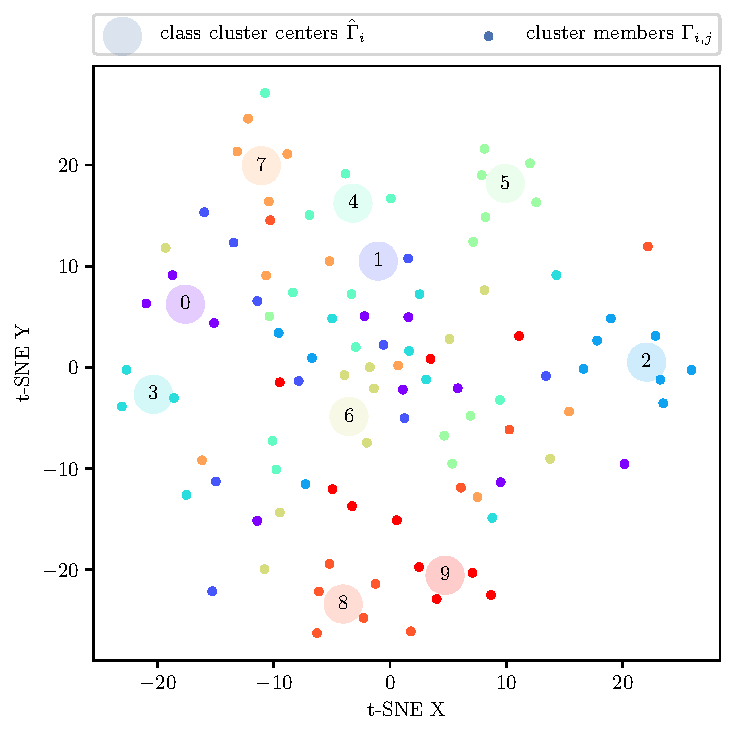
\includegraphics[width=0.36\linewidth]{Appendix_Figures/TSNE_M/new/E-1_gamma_ccp_cluster_pred_fc1.pdf}}
%     \subfigure[\centering\small{Clustering of $\mDelta$ with logits at initialization.}]{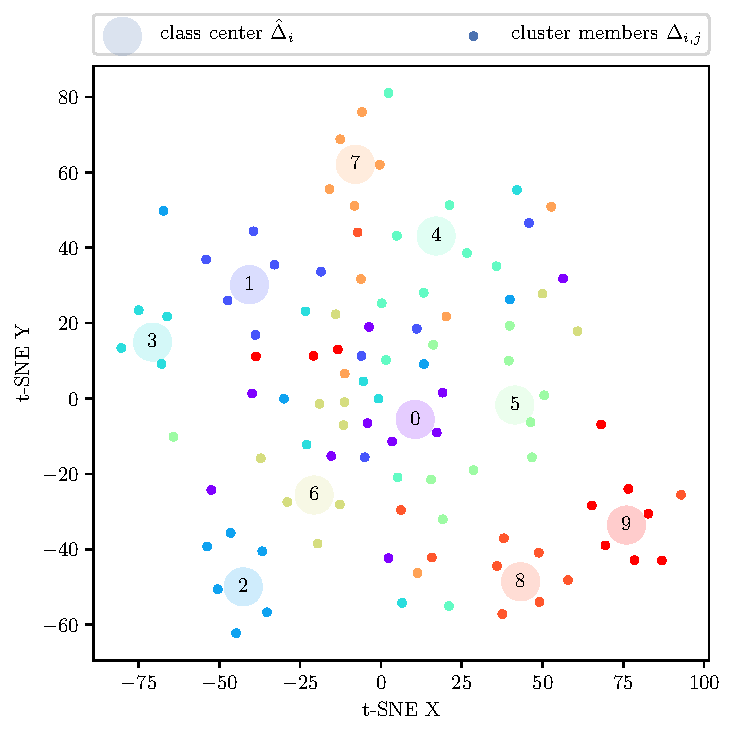
\includegraphics[width=0.36\linewidth]{Appendix_Figures/TSNE_M/new/E-1_delta_ccp_cluster_pred_fc1.pdf}}
%     \caption{Logit clustering behavior of $\mDelta$ and $\mGamma$ at minimum (fc1:T-$200^2$)}
%     \label{fig:tsne2}
% \end{figure}

\begin{figure}[H]
    \centering
    \begin{subfigure}[b]{0.2\textwidth}
        \centering
        \captionsetup{justification=centering}
        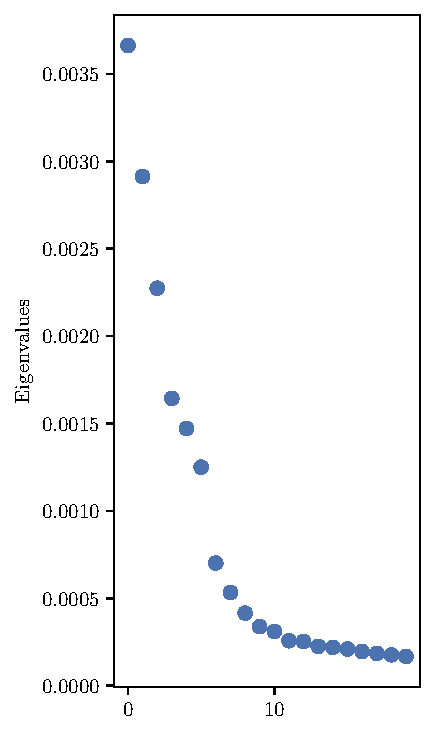
\includegraphics[width=\textwidth]{Appendix_Figures/TSNE_M/new/spec_E-1_gamma_ccp_cluster_pred_fc1.pdf}
        \caption{Eigenspectrum of $\E[\mM]$ at minimum.}
        \label{fig:app_tsne_h_init}
    \end{subfigure}%
    \begin{subfigure}[b]{0.4\textwidth}
        \centering
        \captionsetup{justification=centering}
        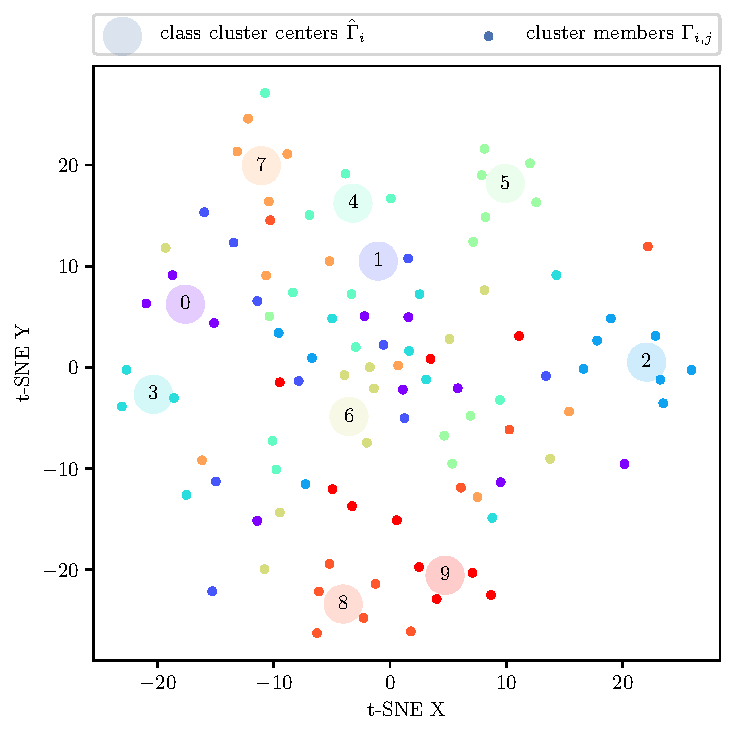
\includegraphics[width=\textwidth]{Appendix_Figures/TSNE_M/new/E-1_gamma_ccp_cluster_pred_fc1.pdf}
        \caption{Clustering of $\mGamma$ with class at minimum.}
        \label{fig:app_tsne_h_min}
    \end{subfigure}%
    \begin{subfigure}[b]{0.4\textwidth}
        \centering
        \captionsetup{justification=centering}
        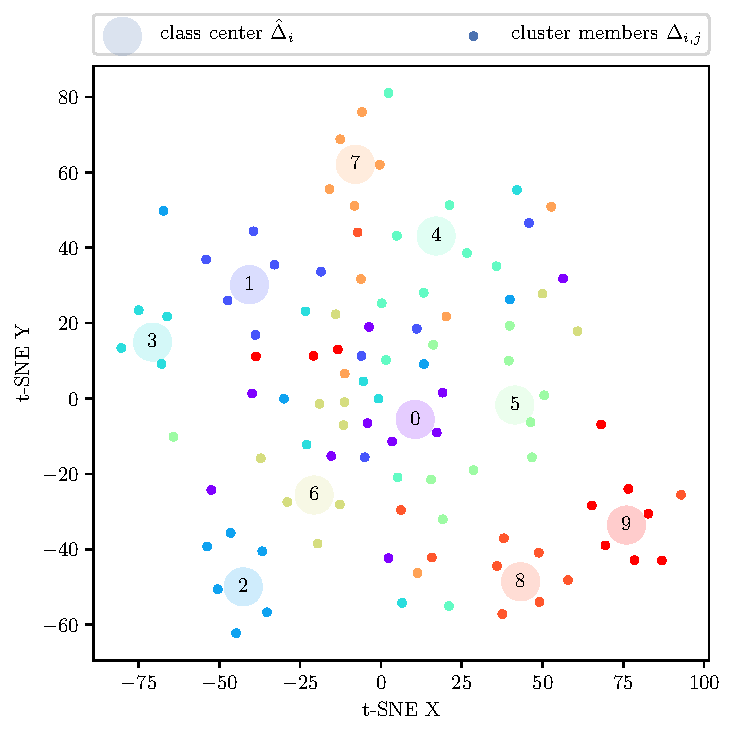
\includegraphics[width=\textwidth]{Appendix_Figures/TSNE_M/new/E-1_delta_ccp_cluster_pred_fc1.pdf}
        \caption{Clustering of $\mDelta$ with class at minimum.}
        \label{fig:app_tsne_m_init}
    \end{subfigure}%
    \captionsetup{justification=centering}
    \caption{Class clustering behavior of $\mDelta$ and $\mGamma$ at minimum. (fc1:T-$200^2$)}
    \label{fig:tsne2}
\end{figure}
